Una vez implementada la funcionalidad de simulación, debe pensarse en añadir una persistencia al proyecto de los elementos que intervienen. Esto es necesario y primordial si se pretende crear una aplicación web para realizar simulaciones. Puesto que se desarrollará una API usando Flask~\cite{Flask} que hará la función de servidor, se ha dedicido utilizar la herramienta para gestión de base de datos SQLAlchemy.
\subsection{Persistencia con SLQAlchemy}
SQLAlchemy~\cite{SqlAl} proporciona un kit de herramientas SQL que permiten manejar bases de datos de manera eficiente. Está formado por dos componentes:
\begin{itemize}
\item \textit{Core}: Es un conjunto de herramientas de SQL que da lugar a un nivel de abstracción sobre el mismo, mediante un lenguaje que utiliza expresiones generativas en Python para expresar órdenes SQL.
\item \textit{ORM}: Se trata de un asignador relacional de objetos, es decir, permite crear una base de datos de objetos virtuales que permite manipular la información de la base de datos, a priori incompatible, como objetos utilizable por un lenguaje de programación orientada a objetos.
\end{itemize}
Mediante las consultas basadas en funciones permite ejecutar las cláusulas SQL a través de funciones y expresiones en Python. Se pueden realizar numerosas acciones como subconsultas seleccionables, insertar, actualizar, eliminar o declarar un objeto, combinaciones internas y externas sin necesidad de utilizar lenguaje SQL. El ORM permite almacenar en caché las colecciones y referencias de objetos una vez han sido cargados, dando lugar a que no sea necesario emitir SQL en cada acceso.\\

SQLAlchemy puede trabajar con bases de datos de SQLite, Postgresql, MySQL, Oracle, MS-SQL, Sybase y Firebird, entre otros.
\subsection{Modelos User y Home}
Se deben determinar los datos que se van a persistir en el sistema. Puesto que se tratará de una aplicación web con la que interactuarán usuarios, resulta interesante almacenarlos. Cada uno de estos usuarios realizará simulaciones del sistema. Como se vió anteriormente, cuando se instancia un objeto de la clase Simulation, el constructor de la misma recibe varios argumentos necesarios para llevar a cabo la simulación, de los cuales la mayoría son información acerca del hogar en el que se realizará dicha simulación (número de módulos fotovoltaicos, código de la ciudad del hogar, etc). La persistencia en base de datos de la información del hogar de cada usuario mejoraría esta situación, pues la mayoría de la información que necesita la clase Simulation sería proporcionada del hogar almacenado en base de datos de ese usuario. Por lo tanto, son necesarias dos tablas en la base de datos: \textit{Users} y \textit{Homes}, entre las cuáles existe una relación \textit{one to one}. Este tipo de relación SQL hace que ambas tablas tengan un atributo de referencia a la otra que se conoce como \textit{\textbf{foreign key}}, la cuál lo convierte en una relación bidireccional. Cada \textit{User} tendrá un \textit{Home} y viceversa. Para crear las tablas y mostrar la estructura lógica de cada una, así como sus limitaciones y atributos, se debe crear antes un \textbf{modelo de base de datos} que sea capaz de \textit{mapear} cada objeto con su tabla en la base de datos.\\

En primer lugar se debe definir la clase Base mediante \textit{sqlalchemy.ext.declarative.declarative\_base()}. Ésta clase hará el papel de superclase de cada modelo. Así, cada modelo heredado de Base corresponde con una tabla de base de datos, cuyo nombre se encuentra en el atributo \textit{\_\_tablename\_\_}. Cada objeto que se instancie la clase del modelo corresponde con un registro en base de datos. En el listado~\ref{lst:declarateModel} se muestra la sintaxis de creación de un modelo. Tras \textit{\_\_tablename\_\_} se declaran las columna que tendrá la tabla de ese modelo, indicando el tipo de dato que contiene y una serie de argumentos. Algunos de los que se han usado son:
\begin{itemize}
       \item \textbf{\textit{primary\_key}:} Cuando toma el valor \textit{True} indica que ese atributo será la clave primaria de la tabla y se usará como parámetro para instanciar a la subclase de Base.
       \item \textbf{\textit{index}:} Con \textit{True} indica que se desea que dicho atributo sea indizado y permita un rápido acceso a los registros.
       \item \textbf{\textit{unique}:} Obliga a que el atributo sea único y no permita registros con el mismo valor en esa columna de la tabla de base de datos.
       \item \textbf{\textit{backref}:} Contiene el nombre de otra tabla en la base de datos. Este argumento permite crear una relación entre ellas.
\end{itemize}
\begin{lstlisting}[language=Python,float=ht,caption={Declaración de un modelo heredado de \textit{Base}},label={lst:declarateModel}]
from sqlalchemy.ext.declarative import declarative_base

Base = declarative_base()

class <Model Name>(Base):
      __tablename__ = <Table Name>
      <attr name> = Column(<data type>, <arg>)
      ...
      ...
\end{lstlisting}
Con la información anterior ya es posible implementar los modelos para las tablas deseadas en el caso particular de este trabajo fin de grado.
\begin{itemize}
\item \textbf{Modelo User}\\
La tabla \textit{Users} hará referencia a los usuarios involucrados en el sistema. Existen una serie de atributos que serán propios de cada usuario y darán lugar a las columnas de la tabla:
\begin{itemize}
\item \textit{name}: Representa el nombre del usuario. Este dato es de tipo String y no puede ser nulo.
\item \textit{lastname}: Representa los apellidos del usuario. Toma exactamente las mismas características que el anterior.
\item \textit{email}: Como su propio nombre indica almacena el correo electrónico del usuario. No puede ser nulo y debe ser único, pues este atributo identificará a cada usuario. Además es un atributo indizado, pues se realizarán consultas a base de datos a través de él.
\item \textit{password}: Contraseña definida por el usuario para acceder a su cuenta. Puesto que la contraseña es un dato sensible, debe tratarse adecuadamente. Para ello se ha hecho uso del módulo \textit{werkzeug.security}, que se explicará en la siguiente sección de este hito en lo relativo a seguridad.
\item \textit{home}: Atributo apunta al registro de la tabla \textit{Homes} que contiene el hogar de este usuario.
\end{itemize}
Véase el listado~\ref{lst:modelUser} el cuál muestra la declaración del modelo \textit{User} heredado de base. Las funciones Integer, String, Column, relationship y declarative\_base son importadas del módulo \textbf{sqlalchemy} y permiten trabajar con abstracción sobre SQL, como se comentó anteriormente. Los métodos de clase \textit{set\_password} y \textit{check\_password} son usados para cambiar y comprobar la contraseña, respectivamente. Ambos llaman a funciones pertencientes al módulo \textit{werkzeug.security} el cuál se explicará más adelante. La función privada \textit{\_\_repr\_\_} simplemente genera un formato para mostrar un objeto Usuario, permitiendo mostrar su nombre, apellidos e email.
\begin{lstlisting}[language=Python,float=ht,caption={Modelo \textit{User}},label={lst:modelUser}]
class Users(Base):
    __tablename__ = 'usuarios'
    id = Column(Integer, primary_key=True)
    name = Column(String(100), nullable=False)
    lastname = Column(String(100), nullable=False)
    email = Column(String(100), unique=True, index=True, nullable=False)
    password_hash = Column(String(128))
    home = relationship("Homes", uselist=False, backref="Users")

    def set_password(self, password):
        self.password_hash = generate_password_hash(password)

    def check_password(self, password):
        return check_password_hash(self.password_hash, password)

    def __repr__(self):
        return (u'<{self.__class__.__name__}: {self.id}, name= {self.name} {self.lastname},' \
                ' email= {self.email}>'.format(self=self))
\end{lstlisting}
\item \textbf{Modelo Home}
La tabla \textit{Homes} representa la casa de cada usuario. Los atributos que tendrá cada registro de esta tabla en base de datos son los siguientes:
\begin{itemize}
\item \textit{city\_code}: Atributo de tipo String que hace referencia a la ciudad donde se encuentra la casa. Esto es necesario a la hora de realizar las llamadas a la API AEMET~\cite{Aemet} pues se debe proporcionar dicho código, por lo tanto este atributo no puede ser nulo.
\item \textit{pv\_modules}: Almacena el número de módulos fotovoltaicos que tendrá el hogar del usuario, por lo tanto es un atributo de tipo Integer que no puede tomar valor nulo, ya que es un dato que determina el resultado de una simulación.
\item \textit{amortization\_years\_pv}: Almacena un entero que representa el número de años en los que el usuario desea amortizar la inversión realizada en la adquisición de los módulos fotovoltaicos. El valor de este campo determina el precio en €/KWh que tendrá la energía fotovoltaica, y por ello tampoco puede ser nulo.
\item \textit{amortization\_years\_bat}: Similar al atributo anterior pero en el contexto de la obtención de la batería. En función del valor de este atributo se calcula el precio que tiene para este usuario la obtención de energía de baterías.
\item \textit{user}: Registro de la tabla \textit{Users} con el que mantiene una relación \textit{one to one} y representa el usuario propietario del hogar.
\end{itemize}
Mediante el método privado \textit{\_\_repr\_\_} se forma un formato para mostrar un registro de esta tabla, dando información acerca de la ciudad, número de módulos fotovoltaicos y id del usuario propietario.
\begin{lstlisting}[language=Python,float=ht,caption={Modelo \textit{Home}},label={lst:modelHome}]
class Homes(Base):
      __tablename__ = "homes"
      id = Column(Integer, primary_key=True)
      city_code = Column(String(100), nullable=False)
      pv_modules = Column(Integer, nullable=False)
      amortization_years_pv = Column(Integer, nullable=False)
      amortization_years_bat = Column(Integer, nullable=False)
      UserId = Column(Integer, ForeignKey('usuarios.id'), nullable=False)
      user = relationship("Users", backref="Homes")

      def __repr__(self):
          return (u'<{self.__class__.__name__}: {self.id}, city= {self.city_code}, ' \
                'pv_modules= {self.pv_modules}, ownerId= {self.UserId}>'.format(self=self))
\end{lstlisting}
\end{itemize}
Una vez definidos los modelos se puede comenzar a realizar inserciones y consultas a estas tablas en la base de datos mediante las operaciones de SQLAlchemy, pero antes se debe comprobar el correcto funcionamiento de estos modelos. Es por esto que la etapa posterior a la implementación en el ciclo de vida del software son las \textbf{pruebas}. Mediante el framework para la implementación de casos de prueba unitarios \textbf{Nose}~\cite{Nose}. Véase el Anexo B, donde se hace referencia a lo relativo a pruebas en el proyecto.\\

Para seguir la guía de buenas prácticas se crean dos bases de datos diferenciadas. Una de ella será la base de datos de \textbf{producción}, que almacenará la información real de usuario y hogares, y será usada por la aplicación web. La segunda será la base de datos de \textbf{test}, donde se realizarán las inserciones, borrados y consultas pertinentes durante el desarrollo de los casos de prueba mencionados anteriormente para garantizar un correcto funcionamiento y coherencia entre la aplicación y la persistencia de la misma.\\

Al arrancar una aplicación que hace uso de la base de datos, se debe hacer una llamada al método \textit{Base.metadata.create\_all} proporcionando como argumento el objeto instanciado de \textit{sqlalchemy.engine.base.Engine}. Esto es necesario ya que permite crear las tablas en la base de datos porporcionada si estas no existen, y si existe, se crearán las nuevas tablas en caso de haberlas y no se eliminan los datos que existen. A partir de dicha llamada, cada objeto que se instancia de cada uno de los modelos se corresponde con un registro de su tabla correspondiente. Después de esto la base de datos estaría totalmente operable desde la aplicación. El ORM de SQLAlchemy permite realizar búsquedas relaccionadas con los objetos instanciados del modelo \textit{Base} y sus tablas relacionadas. Las operaciones se realizan en sesiones, que terminan con un \textit{commit} que persiste los cambios realizados en la sesión en la base de datos. En el listado~\ref{lst:consultaUser} se muestra una consulta para obtener el primer usuario de la tabla \textit{Users}. Nótese que el formato de representación devuelto es el definido en la clase del modelo~\ref{lst:modelUser} mediante el método \textit{\_\_repr\_\_}.
\begin{lstlisting}[language=Python,float=ht,numbers=none,caption={Consulta para obtener el primer \textit{User}},label={lst:consultaUser}]
>>> db.session.query(Users).first()
<Users: 1, name= Pablo Palomino Gomez, email= pablo@eoptimizer.com>
\end{lstlisting}

Para integrar la persistencia que se ha incorporado al funcionamiento actual, debe refactorizarse la clase Simulation. El constructor pasa de recibir un argumento por atributo de clase a recibir únicamente tres atributos: home, user y date. Toda la información necesaria para una simulación que antes se obtenía a través del fichero de constantes del proyecto (y no entendía de usuarios) ahora se puede obtener de los objetos \textit{User} y \textit{Home} del usuario que realiza la simulación. El tercer parámetro (date) hace referencia a un objeto de tipo datetime correspondiente al día en el que se realiza la simulación.\\

A partir de esta integración, se permite realizar simulaciones dependientes de un usuario, que obtendrá un valor totalmente distinto a si otro usuario realiza la simulación el mismo día, pues cada uno de ellos tiene unos parámetros en su hogar que determinan el resultado, como son el número de módulos fotovoltaicos, la ciudad donde reside o el precio al que obtiene las energías fotovoltaica y de batería, ya que cada usuario define el periodo en el que desea amortizar lo invertido en cada fuente mediante ganancias de esa fuente.

\subsection{Creación de una aplicación web con Flask}
El siguiente paso tras la integración de persistencia y la implementación de la lógica o \textit{backend} es crear una aplicación web siguiendo la arquitectura \textbf{cliente - servidor}~\cite{Goer04}. En esta arquitectura, cada una de las máquinas que realiza una demanda de información al sistema toma el rol de cliente, y la que responde a estas demandas toma el rol de servidor~\ref{fig:client-server}. Esto permitirá que exista un servidor el cuál realiza simulaciones a petición de clientes, de los que previamente se ha almacenado la información necesaria en base de datos mediante un registro.
\begin{figure}[!h]
            \centering
            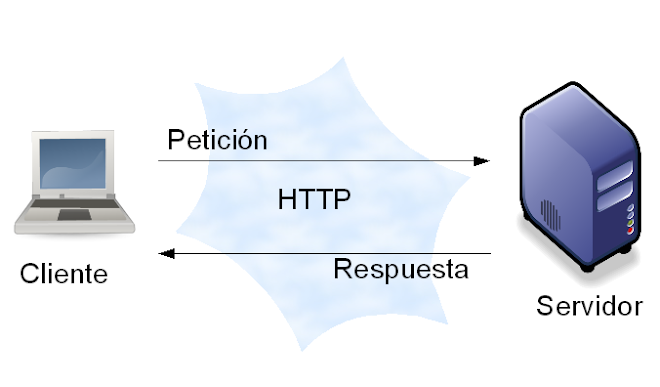
\includegraphics[width=7cm]{figs/client-server.png}
            \caption{Esquema Cliente - Servidor}
            \label{fig:client-server}
\end{figure}
El nombre que tomará dicha aplicación web será \textbf{eOptimizer}, haciendo referencia a su objetivo principal: realizar simulaciones por medio de una optimización. En la figura~\ref{fig:logo} se muestra el logo creado para la aplicación. Dicho logo ha sido diseñado por el propio alumno y se inspira en la eficiencia energética que se consigue mediante el sistema que se propone.
\begin{figure}[!h]
            \centering
            
\includegraphics[width=3cm]{figs/logo.png}
            \caption{Logo de eOptimizer}
            \label{fig:logo}
\end{figure}
Antes de entrar en la implementación de la aplicación debe definirse correctamente el funcionamiento que ha de tener. Esto implica determinar el flujo posible de interación con la aplicación, algo que a la hora de implementar captura de errores y restricciones facilitará mucho la complejidad. Para ello ha de construirse un diagrama de flujo. Este tipo de diagrama describe un sistema informático, y tiene como objetivo planificar, estudiar y diseñar procesos complejos o algoritmos. De entre todas las funcionalidades que pueden implementar los diagramas de flujo, deben mencionarse:
\begin{itemize}
\item Mostrar la ejecución del código de un software.
\item Facilitar la comprensión de la estructura y funcionalidad de una aplicación web.
\item Explicar visualmente cómo un usuario puede navegar por una página web.
\end{itemize}
Para crear un diagrama de flujo debe tenerse en cuenta el alcance del sistema. En el caso de este trabajo fin de grado, un usuario (rol de cliente) interactuará con la aplicación web (servidor) con el objetivo de realizar una \textbf{simulación} del consumo eléctrico de un día determinado que habría tenido su hogar mediante el sistema propuesto, comparándolo frente a su situación actual, por tanto la entrada al diagrama de flujo debe ser el hecho de acceder a la aplicación web, y la salida será la información pertinente a la simulación realizada.\\

Lo primero que debe hacer un usuario es identificarse, pues en el servidor debe tenerse en cuenta el usuario de la base de datos que está interactuando con el sistema para realizar la simulación, ya que necesita su información asociada. Por ello, el usuario deberá introducir sus credenciales para poder acceder. Si un usuario nunca antes ha accedido a eOptimizer, deberá registrarse. Una vez haya introducido la información de usuario para su registro, esta se insertará en base de datos y si todo va correctamente, el siguiente paso es introducir la información asociada a su hogar, que será empleada para realizar sus simulaciones. Cuando se haya introducido se insertará en base de datos, teniendo persistida toda la información necesaria del usuario en curso, por lo que se permitiría el acceso al índice o \textit{dashboard} de la web. Desde allí un usuario podrá realizar simulaciones, introduciendo los datos necesarios para la misma, como son la fecha que desea simular y el fichero de consumo de Endesa que hubo en su hogar ese día. Si esta información es correcta, el \textit{backend} realizará la optimización habiendo obtenido previamente la información de las APIs AEMET y Esios relativa al día de simulación, mostrando los resultados obtenidos al cliente. En la figura~\ref{fig:diagrama-flujo} se muestra el diagrama de flujo de la aplicación que permite visualizar todo el funcionamiento de manera mas sencilla.
\begin{figure}[!h]
            \centering
            \includegraphics[width=15cm]{figs/diagrama_flujo.png}
            \caption{Diagrama de flujo de eOptimizer}
            \label{fig:diagrama-flujo}
\end{figure}
